\documentclass{report}
\usepackage[utf8]{inputenc}
\usepackage{graphicx}
\usepackage{amsmath}
\usepackage{amssymb}
\usepackage{authblk}
\usepackage{caption}

\title{Free Vibration of Cantilever Beam: ME352 Mini Project}

\author[1]{Aditya Shrikhande}	
\author[2]{Drishika Nadella}
\author[3]{Johns Jaison}
\author[4]{Kriti Shukla}
\author[5]{Liz George}

\affil[1]{181ME204, Department of Mechanical Engineering, NITK}
\affil[2]{181ME222, Department of Mechanical Engineering, NITK}
\affil[3]{181ME234, Department of Mechanical Engineering, NITK}
\affil[4]{181ME239, Department of Mechanical Engineering, NITK}
\affil[5]{181ME241, Department of Mechanical Engineering, NITK}

\date{9th April 2021}

\renewcommand\thesection{\arabic{section}}

\begin{document}

\maketitle

\section{Aim}

To find the vibration parameters of the given cantilever beam as well as represent the displacement of the beam with respect to time using a dynamic graph.

\section{Introduction}

If one end of a structure is rigidly fixed to a support and the other end is free to switch, the system is said to be a cantilever beam system. The vibration analysis of a cantilever beam system is crucial because it can clarify and aid in the analysis of a variety of real-world structures.
\bigskip

{\bfseries Natural Frequency of Cantilever Beam}

\bigskip
When a cantilever beam is given an excitation and left to vibrate on its own, it can oscillate at its natural frequency. This is referred to as "free vibration." The value of natural frequency is solely determined by the mass and stiffness of the device. Some assumptions are made for modeling and analysis when a real structure is approximated to a simple cantilever beam: 

\begin{itemize}
 \item At the free end of the beam, the whole system's mass (m) is assumed to be lumped together.
 \item There is no energy-consuming factor in the device (damping), i.e. undamped vibration.
 \item The actual system's complex cross section and material form have been simplified to represent a cantilever beam.
\end{itemize}

The governing equation for such a system (spring mass system without damping under free vibration) is as below:

$$ m \ddot{x} + kx = 0$$

k the stiffness of the system is a property which depends on the length (l), moment of inertia (I) and Young's Modulus (E) of the material of the beam and for a cantilever beam is given by:

$$ k = \frac{3EI}{l^3} $$

\bigskip
{\bfseries Damping in a Cantilever Beam}
\bigskip

Although there is no visible damper (dashpot) the real system has some amount of damping present in it. When a system with damping undergoes free vibration the damping property must also be considered for the modeling and analysis.

Single degree of freedom mass spring damper system under free vibration is governed by the following differential equation:

$$ m \ddot{x} + c\dot{x} + kx = 0$$

$$ \ddot{x} + 2\zeta \omega_n\dot{x} + \omega_n^2x = 0$$

c is the damping present in the system and $\zeta$ is the damping factor of the system which is nothing but ratio of damping c and critical damping $C_c$. Critical damping can be seen as the damping just sufficient to avoid oscillations. At critical condition $\zeta=1$. For real systems the value of $\zeta$ is less than 1. For system where $\zeta$ < 1 the differential equation solution is a pair of complex conjugates. The displacement solution is given by:

$$ x(t) = e^{-\zeta \omega_n t}(x_0 cos(\omega_d t) + \frac{v_0 + \zeta \omega_nx_0}{\omega_d}sin(\omega_d t)$$
 
where $x_0$ and $v_0$ are initial displacement and velocity and $\omega_d$ is the damped natural frequency of the system. The damped natural frequency is calculated as below:

$$ \omega_d = \omega_n \sqrt{1-\zeta^2} $$

\section{Procedure}

In this project, we have created software to simulate the free vibration of a cantilever beam. It is intended for a user who wants to learn the mechanics behind free vibration of cantilever beam interactively. The software allows the user to choose the following values:

\begin{itemize}
    \item Beam length L
    \item End mass of the beam $m_e$
    \item The type of cross-section of the beam. The user can choose from Square, Circular or T-section types. The user can also choose their own custom cross-section. In such a case, they need to input the moment of inertia and the area of cross-section.
    \item The damping factor 
    \item The material of the beam. The user can choose between steel, aluminium and copper.
\end{itemize}

After choosing required values for the above parameters, the following results are displayed:

\begin{itemize}
    \item Natural frequency $\omega_n$
    \item Damped natural frequency $\omega_d$
    \item Damping Ratio $\zeta$
    \item Critical damping coefficient $C_c$
    \item Damping coefficient $c$
    \item Logarithmic Decrement $\delta$
    \item Spring stiffness K
     \item Effective Mass, Meff
\end{itemize}

A displacement vs time graph is also depicted. This helps visualize how the damping factor affects the amplitude of vibration of the cantilever beam over time. The amplitude decreases over time until it becomes zero after a certain time.

\pagebreak

\begin{figure}[!h]
\centering
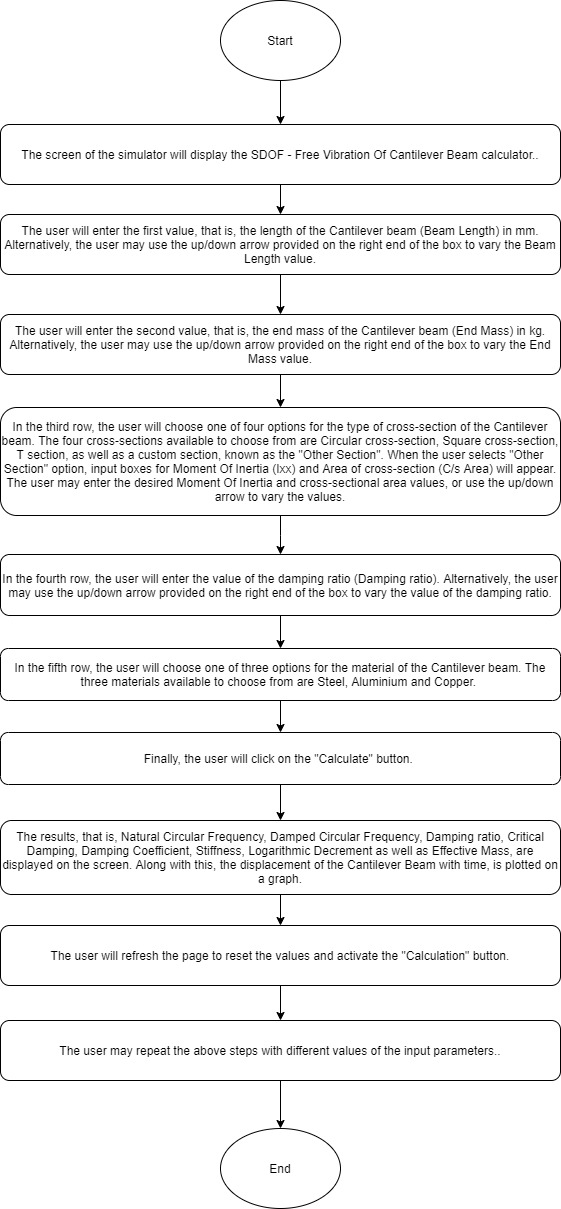
\includegraphics[width=0.6\textwidth]{flowchart.jpg}
\caption{Flowchart depicting the procedure of the SDOF Free Vibration Calculator for Cantilever Beam}
\end{figure}

\pagebreak

\section{Symbols}

\begin{itemize}
    \item $m_b$ = Mass of the beam (kg)
    \item $\rho$ = Density of cantilever beam material $kg/m^3$
    \item $E$ = Young's Modulus of the beam ($m^2$)
    \item $A$ = Area of cross-section of the beam ($m^2$)
    \item $I$ = Moment Of Inertia of the beam ($m^2$)
    \item $m_e$ = End mass (kg)
    \item $m_{eq}$ = Equivalent mass of the beam (kg)
    \item L = Beam length (m)
    \item k = Spring stiffness (N/m)
    \item $\omega_n$ = Natural frequency (rad/s)
    \item $\omega_d$ = Damped natural frequency (rad/s)
    \item $\zeta$ = Damping factor
    \item $C_c$ = Critical damping coefficient (Ns/m)
    \item $C$ = Damping coefficient (Ns/m)
    \item $\delta$ = Logarithmic Decrement 
    
\end{itemize}

For each of the materials considered, we assume the following constants:

{\bfseries Steel:}

\begin{itemize}
    \item Density $\rho$ = 7800 $kg/m^3$
    \item Young's modulus E = 210 Gpa
\end{itemize}

{\bfseries Aluminium:}

\begin{itemize}
    \item Density $\rho$ = 2700 $kg/m^3$
    \item Young's modulus E = 70 Gpa
\end{itemize}

{\bfseries Copper:}

\begin{itemize}
    \item Density $\rho$ = 8940 $kg/m^3$
    \item Young's modulus E = 120 Gpa
\end{itemize}

\section{Equations}

{\bfseries Mass of the cantilever beam:}

$$ m_b = \rho AL $$

{\bfseries Equivalent mass of the beam:}

$$ m_{eq} = 0.23m_b + m_e $$

We multiply the beam mass by a factor of 0.23 because the effective mass of the cantilever beam concentrated at the free end is $0.23m_b$.

\bigskip 

{\bfseries Moment of inertia:}

For a circular cross-section, the moment of inertia I is:

$$I = \frac{\pi d^4}{64}$$

where d is the diameter of the beam.

For a square cross-section, the moment of inertia I is:

$$ I = \frac{a^4}{12} $$

where a is the side length of the cross-section of the beam.

For a T-section, the moment of inertia is:

$$ I = t_1h(y_c-h/2)^2 + t_1h^3/12 + t_2b(h + t_1/2 - y_c)2 + t_2^3b/12 $$

where h = web height, b = flange width, $t_1$ = web thickness, $t_2$ = flange thickness, and $y_c$ = vertical distance of centroid from T-section base.

\bigskip

{\bfseries Area of cross-section:}

\bigskip

For a circular cross-section, the area of cross-section A is:

$$ A = \frac{\pi d^2}{4}$$

where d is the diameter of the beam.

For a square cross-section, the area of cross-section A is:

$$ A = a^2 $$

where a is the side length of the cross-section of the beam.

For a T-section, the area of cross-section A is:

$$ A = bt_1 + ht_2 $$

where h = web height, b = flange width, $t_1$ = web thickness and $t_2$ = flange thickness.

\bigskip

{\bfseries Spring stiffness:}

$$ k = \frac{3EI}{l^3} $$

{\bfseries Natural frequency:}

$$ \omega_n = \sqrt{k/m} $$

{\bfseries Damped natural frequency:}

$$ \omega_d = \omega_n \sqrt{1-\zeta^2} $$

{\bfseries Critical damping coefficient:}

$$ C_c = 2\sqrt{mk} = 2m\omega_n $$

{\bfseries Damping coefficient:}

$$ C = \zeta C_c $$

{\bfseries Logarithmic decrement:}

$$ \delta = \frac{1}{n}log(\frac{x_n}{x_0}) = \frac{2\pi\zeta}{\sqrt{1-\zeta^2}}$$

{\bfseries Displacement vs Time:}

\bigskip

A graph of the displacement of the cantilever beam with respect to the time is displayed along with the results.

This displacement is given by the formula:

$$ x(t) = e^{-\zeta \omega_n t}(x_0 cos(\omega_d t) + \frac{v_0 + \zeta \omega_nx_0}{\omega_d}sin(\omega_d t)$$

where $x_0$ is the initial displacement and $v_0$ is the initial velocity. 

\end{document}
